%------------------------------------------------

\section{Conclusion}
%------------------------------------------------
\begin{frame}[t,label=abm_7]
	\frametitle{Conclusion}
	\tikzstyle{background grid}=[draw, black!50,step=.5cm]
	%
	\uncover<1->{Formulated and solved public health policy-making problems}%
	\only<6->{{\color{white}\ifshowcitations\footpartcite{Ferguson2020}\fi}}\\
	%
	\begin{columns}[t] % The "c" option specifies centered vertical alignment while the "t" option is used for top vertical alignment
		\begin{column}{.42\textwidth} % Left column and width
			\begin{itemize}
				\item<1-> Identified a public health policy that favored
				\begin{itemize}
					\item<2-> High testing capacity $n_T$
					\item<3-> Large number of essential workers $n_E$
					\item<4-> Modest social distancing $S_D$
				\end{itemize}
				\item<5-> StoMADS outperformed GAs and NOMAD on active constraints
				\item<6-> Applicable to other large-scale agent-based models\footnotemark[1]
			\end{itemize}
		\end{column}
		%
		\begin{column}{.5\textwidth} % Left column and width
			\tikzstyle{background grid}=[draw, black!50,step=.5cm]
			\begin{tikzpicture}[remember picture, overlay]%[show background grid]
				\node [inner sep=0pt,above right, opacity=1.0]  at (0.0\textwidth,-0.75\textheight) (mobility) 
				{
					\only<-5>{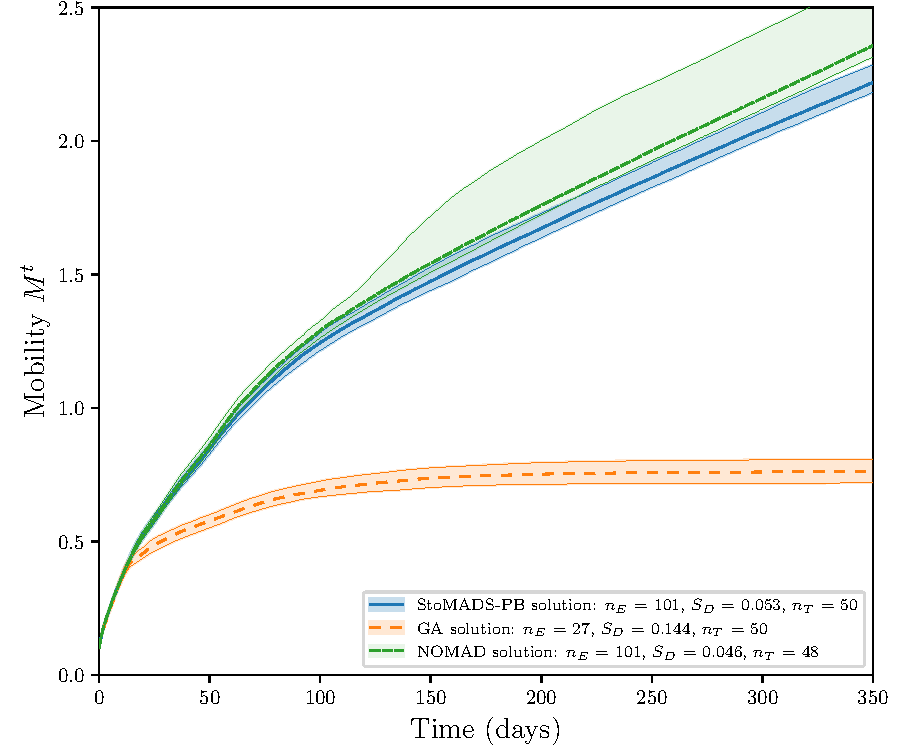
\includegraphics[width=0.93\textwidth]{trajecctory_results/M_compare_opt_2.pdf}}%
				};
				\only<-5>{
					\node[inner sep=0pt,align=flush center,above=\belowcaptionskip of mobility,text width=\linewidth]
					{\vspace{-0em}{
						\large best known solution
					}};
				}%
				% show origin
				% \fill (0,0) circle (2pt);
			\end{tikzpicture}%
			\begin{tikzpicture}[remember picture, overlay] %show background grid, 
				\node [inner sep=0pt,above right, opacity=1.0]  at (0.1\textwidth,-0.66\textheight) (abm) 
					{
						\only<6>{
							\begin{animateinline}[autoplay,width=0.9\textwidth]{8}
								\ifshowanimations
									\multiframe{48}{i=1+15}{%
										\includegraphics{canada_ABM/map_\i.png}
									}
								\else
									\multiframe{1}{i=721+0}{%
										\includegraphics{canada_ABM/map_\i.png}
									}
								\fi
							\end{animateinline}%
						}%
						\only<7->{
							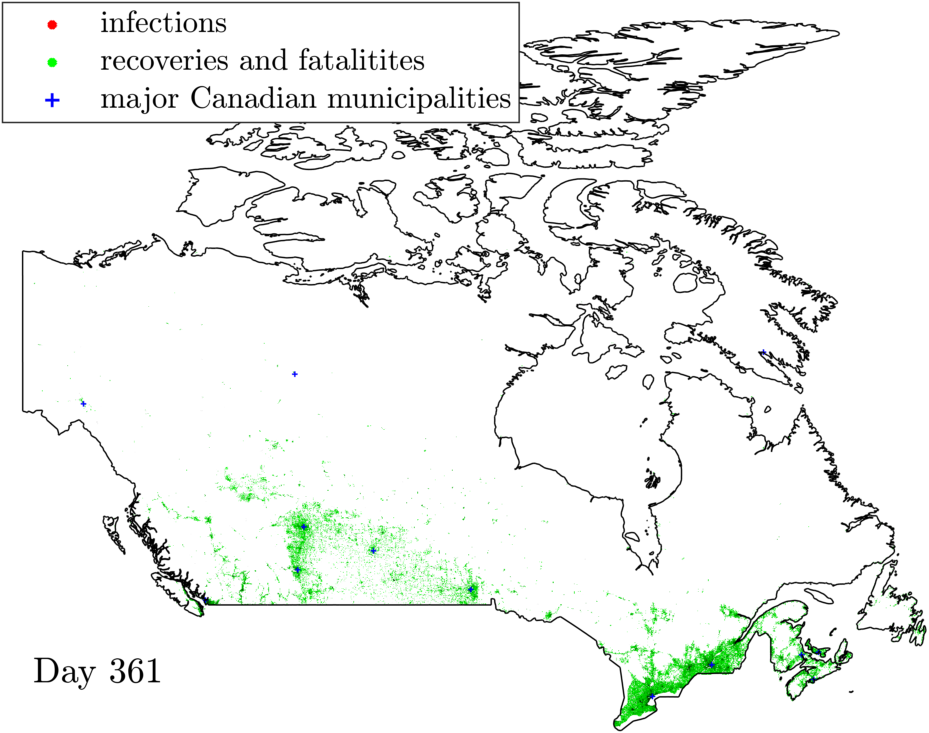
\includegraphics[width=0.9\textwidth]{canada_ABM/map_721.png}
						}
					};
			\end{tikzpicture}%
		\end{column}
	
	\end{columns}
	\vspace{-3em}
\end{frame}
\addtocounter{footnote}{-1}